En esta sección, mostraremos el primer experimento que hicimos. Éste consistió en aplicar un modelo de regresión lineal de cada variable social sobre el \entrainment.

Una variación que usaremos en éste experimento (y en el posterior) es utilizar como variable dependiente el valor absoluto del \entrainment, en base a estudios que sugieren que los interlocutores pueden también diferenciarse como un rasgo positivo en la conversación.

\section{Modelo agrupado o \emph{pooled}}

En el modelo agrupado o \emph{pooled}, no distinguimos entre datos provenientes de distintos ``grupos'' \cite{gujarati1999} y sobre éstos calculamos la regresión lineal, agrupando todos los datos disponibles.

Un problema que surge con este tipo de regresión es que niega todo tipo de \emph{heterogeneidad} de los datos: estos pueden provenir de interlocutores más o menos empáticos, o cuya interacción en el juego se vio influída por factores no medidos en el experimento. Todo ésto es descartado, aún cuando puede afectar seriamente  el resultado obtenido.

\nota{Gráfico de ejemplo de pooled ols}

\begin{figure}[b!]
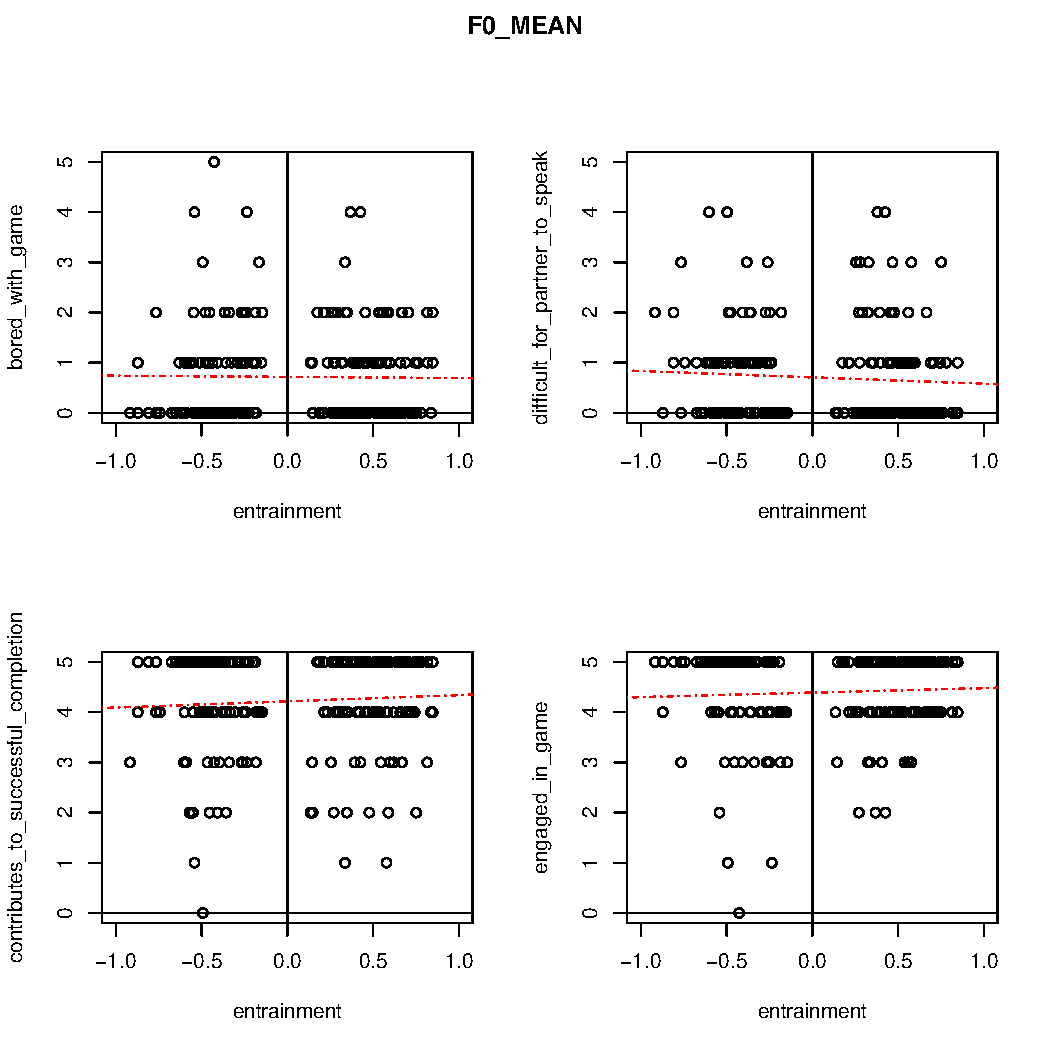
\includegraphics[width=15cm]{images/regression_F0_MEAN_1.pdf}
\caption{Gráfico de los pares entrainment-variable a/p, junto a la regresión lineal obtenida \label{regresion_clasica} para \emph{F0\_MEAN}}
\end{figure}

\section{Resultados sobre \entrainment}

Este modelo dio resultados con baja significancia. En \ref{regresion_clasica} puede verse el gráfico de \emph{F0\_MEAN} y 4 variables sociales y en \ref{regresion_clasica_tabla} pueden verse los valores de las estimaciones de $\estslope$ junto a sus p-valores.

% "ENG_MEAN"
% latex table generated in R 3.2.2 by xtable 1.8-0 package
% Thu Jan  7 03:01:56 2016
\begin{tabular}{rrrrr}
  \hline
 ENG\_MEAN & $\widehat{\beta_2}$ & Std. Error & t value & Pr($>$$|$t$|$) \\
  \hline
  bored\_with\_game & 10.6496 & -0 & 2.036037E-21 & 0.6587 \\
  difficult\_for\_partner\_to\_speak & 10.5625 & -1 & 3.728189E-21 & 0.5893 \\
  contributes\_to\_successful\_completion & 59.6193 & -1 & 9.639522E-133 & 0.2519 \\
  engaged\_in\_game & 73.1439 & 1 & 2.276897E-150 & 0.5851 \\
  gives\_encouragement & 47.4920 & -0 & 1.314327E-113 & 0.9659 \\
  making\_self\_clear & 52.9691 & -1 & 1.022216E-122 & 0.3253 \\
  planning\_what\_to\_say & 32.0193 & -2 & 2.465471E-82 & 0.0718 \\
  dislikes\_partner & 9.6126 & -1 & 2.462398E-18 & 0.3482 \\  \hline
\end{tabular}

% latex table generated in R 3.2.2 by xtable 1.8-0 package
% Fri Jan  8 00:50:24 2016
\begin{tabular}{rrrrr}
  \hline
 ENG\_MAX & $\widehat{\beta_2}$ & Std. Error & t value & Pr($>$$|$t$|$) \\
  \hline
bored\_with\_game & 10.4714 & 0 & 7.003232E-21 & 0.9053 \\
  difficult\_for\_partner\_to\_speak & 10.3984 & -0 & 1.160098E-20 & 0.9678 \\
  contributes\_to\_successful\_completion & 58.9660 & -0 & 8.397021E-132 & 0.6739 \\
  engaged\_in\_game & 72.6730 & 1 & 8.299021E-150 & 0.6008 \\
  gives\_encouragement & 47.3103 & -0 & 2.727411E-113 & 0.6494 \\
  making\_self\_clear & 52.2454 & 1 & 1.465061E-121 & 0.3220 \\
  planning\_what\_to\_say & 31.1729 & 0 & 2.491793E-80 & 0.7176 \\
  dislikes\_partner & 9.5924 & -1 & 2.820254E-18 & 0.3279 \\
   \hline
\end{tabular}

% latex table generated in R 3.2.2 by xtable 1.8-0 package
% Thu Jan  7 03:01:56 2016
\begin{tabular}{rrrrr}
  \hline
F0\_MEAN & $\widehat{\beta_2}$ & Std. Error & t value & Pr($>$$|$t$|$) \\
  \hline
bored\_with\_game & 10.6286 & -0 & 2.355933E-21 & 0.8572 \\
  difficult\_for\_partner\_to\_speak & 10.6764 & -1 & 1.689495E-21 & 0.3316 \\
  contributes\_to\_successful\_completion & 59.3792 & 1 & 2.130619E-132 & 0.3726 \\
  engaged\_in\_game & 73.4118 & 1 & 1.094910E-150 & 0.4425 \\
  gives\_encouragement & 47.5948 & 1 & 8.705216E-114 & 0.2774 \\
  making\_self\_clear & 52.9055 & -0 & 1.290163E-122 & 0.7471 \\
  planning\_what\_to\_say & 31.4874 & 0 & 4.441831E-81 & 0.6977 \\
  dislikes\_partner & 9.8092 & -2 & 6.530815E-19 & 0.0835 \\
   \hline
\end{tabular}

% ""
% latex table generated in R 3.2.2 by xtable 1.8-0 package
% Thu Jan  7 03:01:56 2016
\begin{tabular}{rrrrr}
  \hline
F0\_MAX & $\widehat{\beta_2}$ & Std. Error & t value & Pr($>$$|$t$|$) \\
  \hline
bored\_with\_game & 11.0806 & 2 & 1.001502E-22 & 0.0147 \\
  difficult\_for\_partner\_to\_speak & 10.6511 & 1 & 2.014306E-21 & 0.6023 \\
  contributes\_to\_successful\_completion & 60.0792 & -1 & 2.127331E-133 & 0.3297 \\
  engaged\_in\_game & 74.2016 & -1 & 1.282700E-151 & 0.5711 \\
  gives\_encouragement & 48.1664 & -1 & 8.925956E-115 & 0.2986 \\
  making\_self\_clear & 53.8649 & -2 & 3.954497E-124 & 0.0212 \\
  planning\_what\_to\_say & 31.8577 & -1 & 5.915312E-82 & 0.2950 \\
  dislikes\_partner & 9.6545 & 1 & 1.857261E-18 & 0.3340 \\
  \hline
\end{tabular}



\nota{Mover ésto a antecedentes}
\section{Absolute \entrainment, o \disentrainment}

En nuestra definición de \entrainment en el contexto de series de tiempo, la definimos como el valor de la correlación cruzada (en un sentido de los lags) con mayor valor absoluto. Ésto puede dar, como resultado, valores positivos entre 0 y 1 a los cuales consideramos como \entrainment; o bien valores negativos entre -1 y 0, éstos considerados como anti-\entrainment: la divergencia de las features a/p medidas a través del tiempo.

Este fenómeno de anti-\entrainment o antimimicry \cite{CHAR1999} refiere al proceso por el cual uno de los interlocutores no imita al otro sino más bien todo lo contrario, acentúa alguna diferencia. Si bien estudios de larga data como \cite{bourhis1973language} o \cite{dabbs1969similarity} lo emparentan con una connotación negativa, \cite{healey2014divergence} y \cite{levitan2015acoustic} sugieren que puede entenderse este fenómeno como una conducta de adaptación cooperativa. No sólo éso, sino que este fenómeno de mimetización complementaria es más prevalente que la mimetización a secas \cite{levitan2015acoustic}.

En base a lo recién mencionado es que decidimos probar alguna medida que capture positivamente este fenómeno de igual manera que con el \entrainment definido. Es decir, esperamos que cuando tengamos o bien \entrainment o \entrainment complementario (valores significativos de éste) ocurra que tenemos valores altos de variables sociales de carácter positivo. Mutatis mutandis con las variables sociales de connotación negativa.

Con este fin, en vez de utilizar sólo el valor de \entrainment como variable explicativa, efectuaremos el mismo análisis pero utilizando el valor absoluto del \entrainment como tal. Ésto permite captar y valorar el \entrainment complementario de la misma manera que el ``positivo'' y valorar su relación con las variables sociales medidas.

\section{Resultados sobre \absentrainment}

\nota{Escribir acá, y poner tablas sobre \absentrainment en pooled}

\section{Discusión}

\nota{Vale la pena escribir discusión en pooled?}
